\section{Controllo per il disaccoppiamento di agenti} \label{sec:controllo_accoppiamento_agenti}

L'accoppiamento è un fenomeno causato dalla ridotta distanza tra due o più agenti, e provoca una minore capacità di copertura ed esplorazione da parte dei soggetti coinvolti.
Tale problematica si verifica quando agenti molto vicini identificano ripetutamente la stessa direzione di spostamento, causando un allineamento delle loro traiettorie; questo fa sì che il loro raggio di copertura si riduca a causa delle interferenze mutue.
Ciò ha come effetto quello di restringere l'orizzonte osservabile dagli agenti e conseguentemente un aumento della probabilità che gli agenti selezionino lo stesso punto ottimo.

\begin{figure}[t]
    \centering
    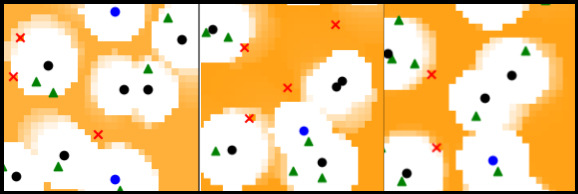
\includegraphics[width=0.8\textwidth]{img/ch3/agent_coupling_event.png}
    \caption[Esempio di accoppiamento tra agenti]{Un esempio di agenti accoppiati, rispettivamente negli istanti 15, 50 e 95. Si vede come, anche se la problematica sembra risolversi alla fine, essa ha drasticamente limitato il contributo degli agenti coinvolti.}
    \label{fig:agent_coupling_event}
\end{figure}

Per cercare di limitare la durata dell'accoppiamento è stato implementata una funzione in grado di riconoscere l'evento ed intervenire, cercando di orientare gli agenti coinvolti in direzioni opposte (Snippet \ref{snip:coupling_detection}).
\pagebreak
L'algoritmo implementato riconosce l'accoppiamento controllando ad ogni iterazione le posizioni pregresse degli agenti, confrontando le distanze mutue con un valore di soglia; nel caso questo venga raggiunto si crea una deviazione che cerca di allontanare gli agenti coinvolti.

\begin{SCfigure}[0.7][h]
    \centering
    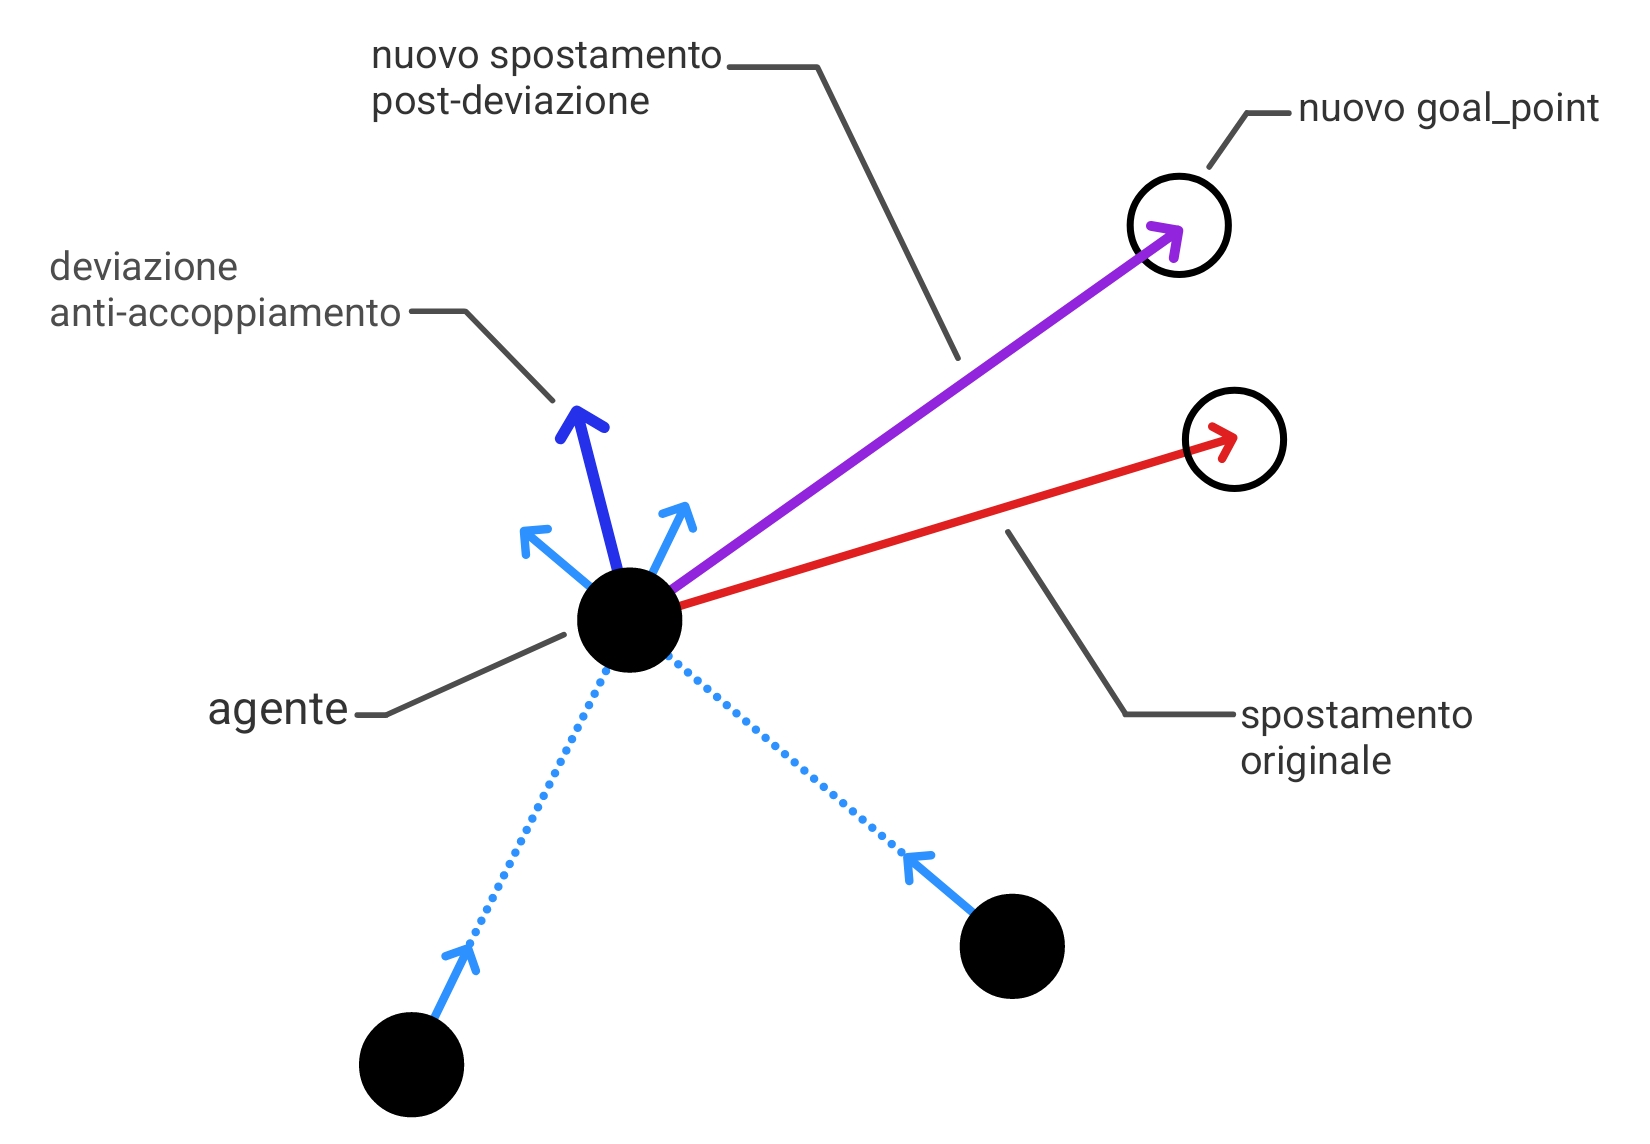
\includegraphics[width=0.6\textwidth]{img/ch3/schematic_anticoupling_system.jpg}
    \caption{Rappresentazione schematica del sistema anti-accoppiamento}
    \label{fig:schematic_decoupling_system}
\end{SCfigure}


Tale deviazione viene applicata sommandola alla direzione di spostamento del punto ottimo, come se fosse presente una forza repulsiva che agisce quando degli agenti sono vicini da troppo tempo (Figura \ref{fig:schematic_decoupling_system}).

\lstinputlisting[
    language=Python 
    , label= {snip:coupling_detection}
    , caption = {Funzione per il riconoscimento dell'accoppiamento.}
    , frame=tb
    , belowcaptionskip=3mm
    , float = p
    ]
{code/coupling_detection_system.py}